\chapter{Was ist KI?}
Um eine \gls{KI} im Bereich des Smart Homes anzuwenden, gilt zunächst die Frage: Was ist \gls{KI} eigentlich? Dabei stehen sich zwei Ansätze gegenüber: Der \textit{menschliche} und der \textit{ideale} Ansatz. Beim menschlichen Ansatz agiert die Maschine wie ein Mensch. Sie hat das Ziel, wie ein Mensch zu denken und zu agieren inklusive des Bewusstseins und emotionalen Verhaltens. Der ideale Ansatz hingegen beschreibt eine Maschine, die rational denkt und sich rational verhält.

\section{Die Theorie}
Der britische Informatiker Alan Turing hat mit seiner Veröffentlichung \enquote{Computing machinery and intelligence} 1950 erstmalig die Begriffe Maschine und Intelligenz in einen Kontext gebracht. Daraus ist die Idee des Turing-Tests entstanden.
\paragraph{Der Turing-Test} ist ein Test um zu überprüfen, ob eine Maschine über menschliche Intelligenz verfügt. Im Szenario des Tests unterhält sich ein Mensch mit Hilfe einer Tastatur und einem Bildschirm mit zwei Gesprächspartnern, wobei einer von ihnen ein Mensch und einer eine Maschine ist. Der Vernehmer kann seine Gegenüber nicht sehen oder hören. Ist der Vernehmer nach einer Reihe von Fragen nicht dazu in der Lage zu unterscheiden, wer Mensch und wer Maschine ist, hat die Maschine den Test bestanden und verfügt über menschliche Intelligenz. Die Maschine kann also einen Menschen \textit{nachahmen}, woraus der ursprüngliche Name des Tests \enquote{The Imitation Game} resultierte.\\\\
Eine ideale \gls{KI} denkt und verhält sich also rational. Diesen Ansatz haben die beiden Informatiker Stuart Russell und Peter Norvig in ihrem Buch \enquote{Artificial Intelligence: A Modern Approach} 1994 vorgestellt. Dabei wird auf die Idee des \enquote{richtigen Denkens} eingegangen, die initial vom griechischen Philosophen Aristoteles entworfen wurde. Das Ziel ist es, Entscheidungen nicht emotional beeinflussen zu lassen, wie es bei einem Menschen der Fall wäre.

\section{Die praktische Umsetzung}
Die theoretischen Ansätze der Funktionsweise von \glspl{KI} sind Modelle, die sich nicht eins zu eins praktisch umsetzen lassen. Als Abhilfe gibt es in der Praxis mehrere Ansätze eine \gls{KI} zu modellieren und umzusetzen.

\subsection{if: then - Ansatz}
Der if: then - Ansatz beschreibt die simpelste Art von Intelligenz, die ein Programm aufweisen kann. Hierbei wird davon ausgegangen, dass es als Intelligent erachtet wird, wenn ein Programm eigenständig eine Aufgabe lösen kann, die für einen Menschen gedacht ist. Oft werden mit diesem Ansatz \glspl{KI} für sehr einfache Spiele entwickelt.

\begin{figure}[htbp]
    \centering
    \fbox{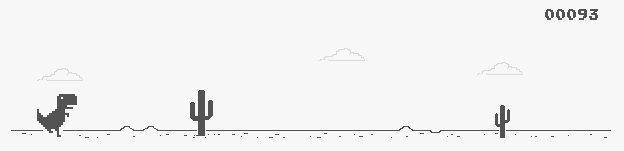
\includegraphics[width=\textwidth]{img/trex_game}}
    \caption{\label{fig-trex}Steve the Jumping Dinosaur - Spiel}
\end{figure}

Beispiel: \enquote{Steve the Jumping Dinosaur} ist ein Spiel, bei dem der Spieler einen kleinen Dinosaurier steuert. Dieser muss über Kakteen springen und läuft dabei kontinuierlich nach rechts, wobei immer neue Kakteen erscheinen, die überwunden werden müssen (siehe \cref{fig-trex}).\\
Um das Spiel von einer \gls{KI} steuern zu lassen, reicht es aus, die Pixel mit ein wenig Abstand vor dem Dinosaurier abzutasten, und zu überprüfen, op ein Kaktus vorhanden ist oder nicht. Dazu muss der Pixel vor dem Dinosaurier einen bestimmten Wert (Threshhold) übersteigen. Dies muss jedes mal geschehen, wenn ein neuer Pixel am Spielrand angezeigt wird. Der Code-Auszug \ref{algo-dino-game} zeigt solch eine Implementierung in drei Zeilen, wobei die Funktionalitäten zum Pixelwert lesen und Ausführen des Sprungs ausgelagert sind. Es wird davon ausgegangen, dass diese Funktion jedes mal aufgerufen wird, wenn sich der Dinosaurier bewegt.

\begin{lstlisting}[language=python,
frame=single,
framexleftmargin=15pt,
style=algoBericht,
label={algo-dino-game},
captionpos=b,
caption={Dinosaurier-Spiel KI}]
def game_loop():  # hauptfunktion, die zu jedem Spiel-Tick ausgefuehrt wird
    if get_greyscale(200, 30) > 50:  # Grauwert des Pixels vor dem Dino ueberpruefen
        perform_jump()
\end{lstlisting}

Der Anwendungsfall kann dabei jedoch auch sehr Komplex werden. Nach dieser Art eine \gls{KI} für z. B. Tetris zu entwickeln, wird etwas komplexer. Grundlagen dieses Ansatzes ist es also, dass der Entwickler jede Eventualität, die eintreffen könnte, bei der Entwicklung berücksichtigt. In Bezug auf die Steuerung von Gebäudetechnik wäre ein Anwendungsbeispiel: Wenn die Sonne untergeht, mach das Rollo runter.\\
Dieser Ansatz wird in dieser Arbeit verwendet.

\subsection{Künstliche Neuronale Netze}
Ein \gls{KNN} soll einer Abbildung des menschlichen Gehirns als mathematisches Zahlenmodell ähneln (\cref{fig-knn}).

\begin{figure}[htbp]
    \centering
    \fbox{\includegraphics[width=0.72\textwidth]{img/künstliche-neuronale-Netze.jpg}}
    \caption{\label{fig-knn}Künstliches Neuronales Netz}
\end{figure}

Die Grundidee von \glspl{KNN} ist es, dass die Knoten in \Cref{fig-knn} die Neuronen und die Kanten die Synapsen, also die Verbindung zwischen zwei Neuronen, darstellen. Die Daten, aus denen eine Ausgabe erzeugt werden soll, werden den Eingabeneuronen zugeordnet. Das \gls{KNN} betrachtet die Eingabe als beliebige, einheitslose Zahlenwerte. Die Zahlenwerte gehen von der Eingabeschicht auf die verborgene Schicht über und werden an jedem der Knoten in dieser Schicht zu einer neuen Zahl aufsummiert. Auf dem Weg zum neuen Knoten wird die Zahl durch eine Gewichtung auf den Kanten verändert. Jede Kantengewichtung ist unabhängig voneinander. Von der verborgenen Schicht, die sich beliebig oft in verschiedenen Größen wiederholen kann, gehen die Zahlenwerte letztendlich auf die Ausgabeschicht über. Ein Anwendungsbeispiel mit dem gegebenen \gls{KNN} kann sein: Ein Roboterauto verfügt über drei Abstandssensoren (vorne rechts, vorne mittig und vorne links). Diese Werte werden in das \gls{KNN} aus \Cref{fig-knn} eingespeist und die Ausgabe bewertet, wie stark das Auto nach rechts oder links lenken soll. Ist das \gls{KNN} mit den Gewichtungen optimiert, so kann das Auto unfallfrei fahren.\\